
\TChapter{Marco teórico}{gama}
\ \\\\
En esta sección se expondrán de manera detallada conceptos los cuales son esenciales para la elaboración de este trabajo.

%Recordar renombrar las citas
\section{Inteligencia Artificial}
La Inteligencia Artificial (AI) es un campo de investigación y desarrollo que tiene por objetivo 
resolver problemas complejos para los cuales no se conocen soluciones algorítmicas exactas 
computables en la práctica, ya sea por sus grandes dimensiones, su complejidad estructural o los 
niveles intrínsecos de incertidumbre de los datos que manejan \citep{CT1}.
\\
Hoy en día la Inteligencia Artificial juega un papel muy importante en el desarrollo diversos 
campos de investigación, así como en la industria, finanzas, educación, transporte y más.
\\
La tecnología ha avanzado día con día y eso implica que la Inteligencia Artificial también avanza, 
uno de los objetivos primordiales de la Inteligencia Artificial es construir modelos computacionales 
capaces de resolver las actividades que realiza el ser humano de una manera más eficiente y precisa.


\section{Machine Learning}

Machine Learning es una rama de la Inteligencia Artificial la cual permite  desarrollar técnicas aprendizaje 
automático por parte de las computadoras, los cuales tienen la capacidad de resolver problemas, predecir 
continuamente los cambios que se puedan suscitar, gracias a los modelos de aprendizaje utilizados en ellos.
\\\\
Machine Learning utiliza una variedad de algoritmos que aprenden iterativamente de datos para mejorar, describir 
datos y predecir resusltados. A medida en la cual los algoritmos de entrenamiento obtienen datos es posible obtener 
modelos más precisos basados en esos datos. Un modelo de Machine Learning es una salida generada cuando se tiene 
entrenado un algoritmo de aprendizaje automático. Después de entrenar el modelo con una entrada de datos, obtendremos 
una salida. Por ejemplo, un algoritmo predictivo creará un modelo predictivo. Luego, cuando se le proporciona datos 
al modelo predictivo, se obtendrá una predicción basada en los datos que entrenaron al modelo \citep{CT2}.
\\
%https://www.ibm.com/downloads/cas/GB8ZMQZ3
%Machine Learning es un método de análisis de datos el cual permite automatizar la obtención de 
%resultados a partir de una numerosa cantidad de datos. Es una disciplina de la Inteligencia 
%Artificial la cual permite optimizar operaciones, realizar predicciones basadas en la información 
%que se le proporcione.
\\
Algunas de las áreas en las cuales Machine Learning se ha visto involucrada es \citep{CT3}:
\begin{itemize}
	\item Servicios financieros: Las empresas pueden detectar insights en la información de sus clientes 
	y sus operaciones, permitiendo de manera automatizada la recomendacion de productos financieros al usuario 
	indicado y en el momento preciso.
	\item Salud: En combinación con sensores o dispositivos en prendas de vestir (weareble devices) 
	un sistema puede monitorear y valorar el estado de salud de una persona en tiempo real, y si detecta 
	una irregularidad, tomar una acción en forma automática.
	\item Ventas y mercadotecnia: A partir de compras previas por el usuario se pueden realizar 
	realizar recomendaciones con alto potencial de éxito. Este conocimiento del cliente también ayuda a implementar 
	campañas de marketing con gran nivel de precisión.
	\item Gobierno:  El gobierno puede analizar su gigantesco cúmulo de datos, y detectar ágilmente áreas o
	funciones cuya mejora debe ser prioritaria –de esta forma, los recursos	públicos se invierten en los ámbitos 
	correctos, aquellos que realmente mejoran la vida de la ciudadanía y evitan procesos lentos y burocráticos.
	\item Transporte: Las compañías analizan sus operaciones de negocio y rápidamente detectan rutas más
	eficaces, lo que incrementa la rentabilidad de sus procesos (tiempos de entrega más cortos, con menor consumo 
	de combustible, menor riesgo de desperfectos y menor desgaste de las unidades).
\end{itemize}

\subsection{Aprendizaje supervisado}
Los algoritmos de aprendizaje supervisado dependen de datos previamente etiquetados, es decir necesita de un entrenamiento para 
que el algoritmo pueda comprender los datos y con ello determinar que etiqueta debe asignarse a los nuevos datos 
en función del patron y asociando los patrones a los nuevos datos sin etiquetar. Después de ello, la maquina recibe 
un nuevo conjunto de datos para que el algoritmo de aprendizaje supervisado analice los datos y produzca un resultado 
correcto de los datos etiquetados \citep{CT4}.

\subsubsection{Regresión líneal}
La regresión es una técnica estadística utilizada para estudiar la relación entre dos variables, permite hallar el valor esperado de 
una variable aleatoria a cuando b toma un valor específico. La aplicación de este método implica un supuesto de linealidad cuando 
la demanda presenta un comportamiento creciente o decreciente, por tal razón, se hace indispensable que previo a la selección de 
este método exista un análisis de regresión que determine la intensidad de las relaciones entre las variables que componen el modelo.
\\
El pronóstico de regresión lineal simple es un modelo óptimo para patrones de demanda con tendencia (creciente o decreciente), 
es decir, patrones que presenten una relación de linealidad entre la demanda y el tiempo \citep{CT5}.

La figura \textbf{\ref{fig:RL}} muestra un ejemplo de los resultados obtenidos utilizando regresión líneal. 

\begin{figure}[H]
  \centering
  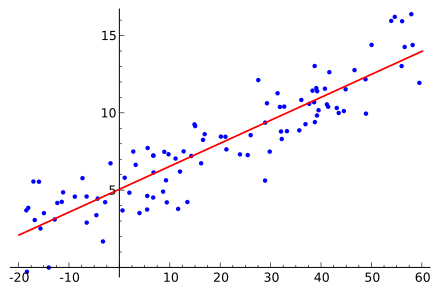
\includegraphics[scale=.6]{imagenes/Capitulo3/regresionLineal}
  \caption{Regresión lineal con una variable dependiente y una variable independiente.}
  \label{fig:RL}
\end{figure}
%https://cleverdata.io/conceptos-basicos-machine-learning/

\subsubsection{Regresión logística}
La regresión logística es una técnica estadística multivariante que nos permite estimar la relación existente entre una variable dependiente 
no métrica (donde la variable es binaria o también conocida como dicotómica, es decir, solo va a dar como resultado dos alternativas posibles) 
y un conjunto de variables intependientes métricas o no métricas \citep{CT6}. Es útil para modelar la probabilidad de un evento ocurriendo como 
función de otros factores. El análisis de regresión logística se enmarca en el conjunto de Modelos Lineales Generalizados que usa como función de 
enlace la función logit. Las probabilidades que describen el posible resultado de un único ensayo se modelan, como una función de variables explicativas, 
utilizando una función logística.

La regresión logística es usada extensamente en las ciencias médicas y sociales. Otros nombres para regresión logística usados en varias áreas de 
aplicación incluyen modelo logístico, modelo logit, y clasificador de máxima entropía.


\subsubsection{Na{\"i}ve bayes}
Na{\"i}ve Bayes es un conjunto de algoritmos de aprendizaje supervisado que se basan en la aplicación del teorema de Bayes con "Na{\"i}ve" 
(Ingenuo) la cual es la supuesta de independencia condicional entre cada par de características dado el valor de la variable de clase. 

La clasificación Naive Bayes son aproximaciones probabilísticas, las cuales hacen especulaciones sobre como deben de ser 
generados los datos. Generalmente utilizan aprendizaje supervisado sobre el conjunto de entrenamiento para poder esimar los parámetros 
del modelo generativo, en tanto el conjunto de datos de entrada nuevos se realiza el teorema de Bayes, seleccionando la probable categoría 
que se ha generado \cite{CT7}.
\\
Todas las características extraídas que utilizan este clasificador son independientes entre sí. La ventaja de usar este clasificador es que 
funciona bien tanto con datos numéricos como con datos textuales y, además, es más fácil de implementar. La desventaja de este clasificador es 
que su rendimiento empeora cuando las características extraídas se correlacionan entre sí.

\subsubsection{Maquina de soporte vectorial}
Las maquinas de soporte vectorial son un conjunto de algoritmos de aprendizaje los cuales se basan en el uso de un espacio de funciones lineales, 
el cual se encuentra con mas dimensiones inducido por un kernel, en el que las hipotesis son las entradas para el algoritmo. \\
El algoritmo induce separadores lineales ya sea en el espacio original de los ejemplos de entrada, si los datos no son separabales se busca un hiperplano 
en el que si lo sean, se hace de forna implicita con las funciones kernel.\\

Estos métodos están propiamente relacionados con problemas de clasificación y regresión. Dado un conjunto de ejemplos de entrenamiento (de muestras) 
podemos etiquetar las clases y entrenar una SVM para construir un modelo que prediga la clase de una nueva muestra. Intuitivamente, una SVM es un modelo 
que representa a los puntos de muestra en el espacio, separando las clases a 2 espacios lo más amplios posibles mediante un hiperplano de separación definido 
como el vector entre los 2 puntos, de las 2 clases, más cercanos al que se llama vector soporte. Cuando las nuevas muestras se ponen en correspondencia con dicho 
modelo, en función de los espacios a los que pertenezcan, pueden ser clasificadas a una o la otra clase \citep{CT8}.

\subsubsection{Random forest}
Random forest es una combinación de árboles predictiroes, de modo que cada árbol depende de los valores de un vector 
aleatorio muestreado independientemente y con la misma distribución para cada uno de estos. Es una modificación sustancial de bagging que construye una 
larga colección de árboles no correlacionados y posteriormente los promedia \citep{CT9}.

\subsection{Aprendizaje no supervisado}
Los algoritmos de aprendizaje no supervisado no dependen de datos previamente etiquetados, por lo cual los algoritmos 
tienen la tarea de agrupar la información no clasificada según sus similitudes, patrones y diferencias sin ningún entrenamiento 
previó de datos, por lo cual aprenden gracias a la cantidad de datos que le son ingresadas con características propias de un 
objeto y con ello pueda determinar los resultados basados en los datos de entrada \citep{CT10}.
%https://towardsdatascience.com/supervised-machine-learning-classification-5e685fe18a6d

\section{Procesamiento de lenguaje natural}
El procesamiento de lenguaje natural es una disciplina de la Inteligencia Artificial que se ocupa de la formulación e 
investigación de mecanismos computacionales para la comunicación entre personas y maquinas mediante el uso de Lenguajes 
Naturales[16].

%\subsection{Lenguaje}
%El lenguaje es un medio de comunicación a traves de de un sistema de símbolos \cite{dieciseis}.
%La Real Academía Española define al lenguaje como la facultad del ser humano de expresarse y comunicarse con los demás 
%a través del sonido articulado o de otros sistemas de signos.


\subsection{Tokenización}
Es la acción de separar el texto en sus unidades míninas(Palabras), se les
asigna un código como el ascii o hexadecimal para ser reconocidas de fórma
única, son almacenas para su postrior análisis y reconocimiento. Cabe mencionar que los
signos de puntuación son eliminados.

\subsection{Lematización}
Es el proceso lingüstico que, dada una palabra flexionada se encuentra su
lema. Una palabra flexionada es cuando esta en el plural, en femenino conjugada,
diminutivo o en superlativo. El lema es la palabra que esta en singular para
sustantivo, singular masculino para adjetivo e infinitivo para un verbo. Ejemplo:

	\begin{itemize}
		\item amigos, amiga, amiguitos-> Amigo
		\item soy, son, es->Ser
	\end{itemize}

Cabe mencionar que existen diversos grados de lemataizaicón

	\begin{itemize}
		\item Mórfólogica: Es la anterior mente explicada
		\item Sintáctica: Toma encuenta el contexto donde se encuentra la palabra

	\end{itemize}

Una opción para lematizar es Freeling, este es un lematizador hecho por la
universidad de catalunia.

\section[Representación del t.]{Representación del texto}
Los métodos de aprendizaje automático, requieren que la información este
representado en un formato que facilite su procesamiento. Un método utilzado
es representar los datos en un vector de valores numéricos.

\section{Corpus}
Se le llama corpus a la recopilación de un conjunto de textos, de materiales escritos y/o hablados, 
agrupados bajo un conjunto de criterios mínimos, para realizar ciertos análisis lingüísticos.



\section{Crawler}
Un crawler \cite{once} es una herramienta la cual analiza sitios web, permitiendo recolectar 
las páginas web para así posteriormente extraer la información que contengan. Un crawler también 
conocido como como robot o spider, es un sistema para la descarga masiva de páginas web. Son uno de 
los componentes principales de los motores de búsqueda web, los sistemas que reúnen un conjunto de 
páginas web, las indexan y permiten a los usuarios realizar consultas contra el índice y encontrar las 
páginas web que coincidan con las consultas.


\section{Sitios web}
Un sitio web \cite{doce} es un conjunto de páginas web interconectadas y de acceso público que comparten 
un solo nombre de dominio. Los sitios web pueden ser creados y mantenidos por un individuo, grupo, empresa 
u organización para cumplir una variedad de propósitos. Todos estos sitios constituyen la World Wide Web. 

\subsection{Página web}
Una página web es un documento electrónico el cual forma parte de la WWW (\textit{World Wide Web}) generalmente 
construido en el lenguaje HTML (\textit{Hyper Text Markup Language}). Este documento puede contener enlaces que nos 
direcciona a otra página web. Para visualizar una página web es necesario de un browser o un navegador \cite{trece}. 
Dentro de las páginas web podemos encontrar un sinfin de sitios los cuales pueden ser de nuestro interés.

\subsection{Blog}
Un blog es una página web en la cual el usuario no necesita conocimientos específicos del medio electrónico ni del 
formato digital para poder aportar contenidos de forma inmediata, ágil y constante desde cualquier punto de conexión 
a Internet \cite{catorce}. En un blog el usuario puede compartir cualquier tipo de información que sea de su agrado, 
teniendo una mayor libertad de expresión lo cual permite que otras personas compartan y comenten su manera de expresarse.

\subsection{Foro}
Un foro es una herramienta de comunicación asíncrona. Los foros permiten la comunicación de los participantes desde 
cualquier lugar en el que  esté  disponible  una  conexión  a Internet  sin  que  éstos  tengan  que  estar dentro del 
sistema al mismo tiempo, de ahí su naturaleza asíncrona \cite{quince}. Brindando una mayor interacción entre distintos 
participantes y permitiendo conocer la opinión sobre un tema de distintas personas.


